% prelab3
\documentclass{IEEEtran}
\usepackage{booktabs}
\usepackage{graphicx}
\usepackage{fancyhdr}
\usepackage{framed}
\usepackage{siunitx}
\usepackage{amsmath}
\pagestyle{fancy}
\lhead{}
\chead{}
\rhead{}
\lfoot{}
\cfoot{}
\rfoot{\thepage}
\title{Prelab 2 Amplifiers}
\author{Group 8: Muhan Li \and Man Sun \and Mingxiao An \\ EE233 Circuit Theory}
\IEEEaftertitletext{\centering \vspace{-10pt} \fontsize{11}{11}\textsc{Department of Electrical Engineering, University of Washington, Seattle, WA, 98195} \vspace{10pt}}
\begin{document}
	\maketitle
	\section{\textbf{Prelab\#1}}
	\begin{equation*}
		H(\mathbf{j}\omega) = \frac{V_{out}}{V_{in}} = -\frac{R_f}{R_s}
	\end{equation*}
	\phantom{ } As the result shows, the frequency response of the circuit is obviously a negative number, which means the amplifier inverts the positive and negative of the input voltage.\\
	\section{\textbf{Prelab\#2}}
	\begin{equation*}
		\mathrm{gain} = | H(\mathbf{j}\omega) | = -\frac{R_f}{R_s} = -47
	\end{equation*}
	which means that we need to choose two resistors and one is 47 times in resistance of the other. From the lab kit, we choose a 47$ \si{k\Omega} $ resistor and a 1$ \si{k\Omega} $ resistor. Our schematic is shown in graph[\ref{fig:201}].
	
	\begin{figure}[!htbp]
		\centering
		\begin{framed}
			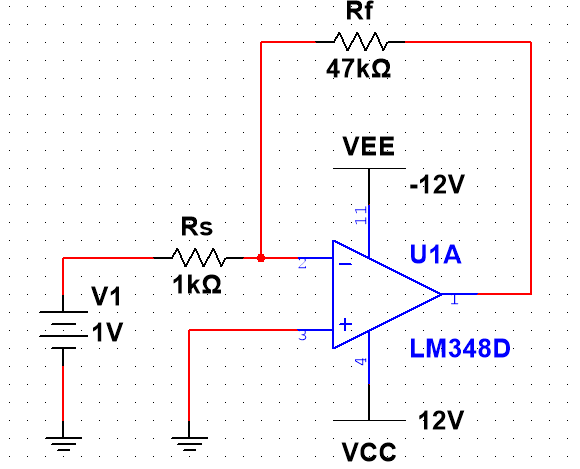
\includegraphics[width=\linewidth]{images/2_1.PNG}
			\caption{Output impedance}
			\label{fig:201}
		\end{framed}
	\end{figure}

	\section{\textbf{Prelab\#3}}
	\subsection{the Matlab Bode plot}
	\begin{figure}[!htbp]
		\centering
		\begin{framed}
			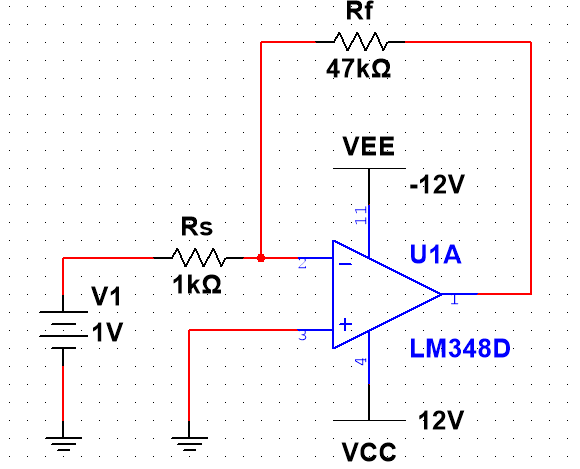
\includegraphics[width=\linewidth]{images/2_1.PNG}
			\caption{the Matlab Bode Plot for prelab \#3}
			\label{fig:301}
		\end{framed}
	\end{figure}
	\subsection{the SPICE Bode plot}
	
	\section{\textbf{Prelab\#4}}
	\begin{eqnarray*}
		\frac{V_{in}}{R_s} & = & \frac{V_{out}}{R_s + R_f}\\
		H(\mathbf{j}\omega) & = & \frac{V_{out}}{V_{in}} = \frac{R_s+R_f}{R_s}\\
	\end{eqnarray*}
	We can see that the response is always a positive constant, so the output isn't inverted by the op amp, which is why it is known as a non-inverting amplifier.
	
	\section{\textbf{Prelab\#5}}
	\begin{eqnarray*}
		\frac{R_s+R_f}{R_s} & = & 48\\
		R_s & = & 1\si{k\Omega}\\
		R_f & = & 47\si{k\Omega}\\
	\end{eqnarray*}
	So we choose the same two resistors as in prelab \#2. The schematic graph is shown in figure[\ref{fig:501}].
	
	\begin{figure}[!htbp]
		\centering
		\begin{framed}
			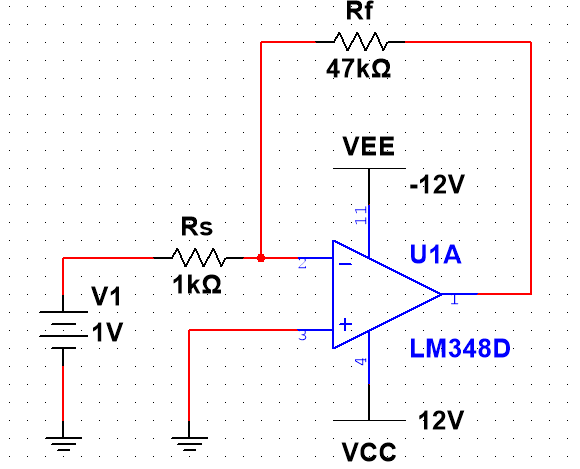
\includegraphics[width=\linewidth]{images/2_1.PNG}
			\caption{Output impedance}
			\label{fig:501}
		\end{framed}
	\end{figure}

	\section{\textbf{Prelab\#6}}
	\subsection{the Matlab Bode Plot}
	\begin{figure}[!htbp]
		\centering
		\begin{framed}
			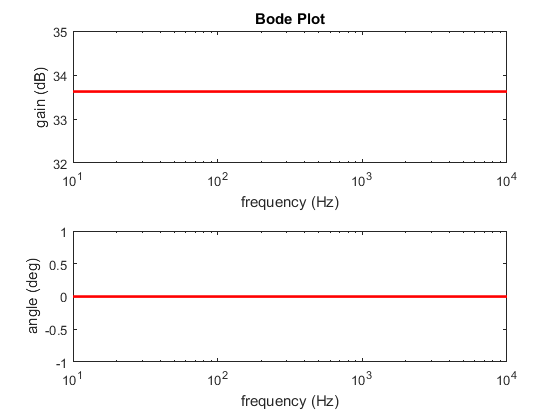
\includegraphics[width=\linewidth]{images/6.png}
			\caption{the Matlab Bode Plot for prelab \#6}
			\label{fig:301}
		\end{framed}
	\end{figure}

	\subsection{the SPICE Bode Plot}
	
	\section{\textbf{Prelab\#7}}
	\begin{eqnarray*}
		\frac{V_{in}}{R_s} & = & -\frac{V_{out}}{\frac{1}{\mathbf{j}\omega C}}\\
		H(\mathbf{j}\omega) & = & \frac{V_{out}}{V_{in}} = -\frac{1}{\mathbf{j}\omega CR_s}\\
	\end{eqnarray*}
	%TODO
	\section{\textbf{Prelab\#8}}
	
	\section{\textbf{Prelab\#9}}
	\subsection{the Matlab Bode Plot}
	\begin{figure}[!htbp]
		\centering
		\begin{framed}
			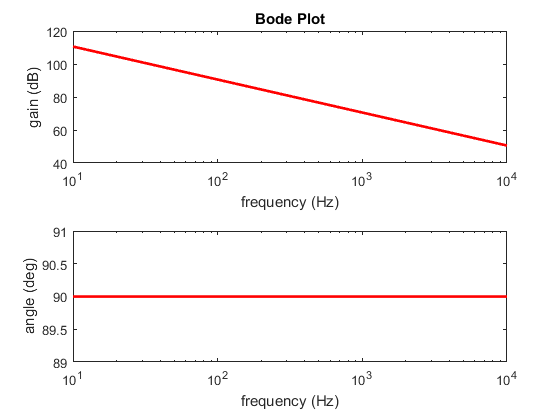
\includegraphics[width=\linewidth]{images/9.png}
			\caption{the Matlab Bode Plot for prelab \#9}
			\label{fig:901}
		\end{framed}
	\end{figure}
	\subsection{the SPICE Bode Plot}
	
	\section{\textbf{Prelab\#10}}
	\subsection{the frequency response}
	\begin{eqnarray*}
		\frac{V_{in}}{R_s} & = & -\frac{V_{out}}{\frac{1}{\mathbf{j}\omega C}} - \frac{V_{out}}{R_f}\\
		H(\mathbf{j}\omega) & = & \frac{V_{out}}{V_{in}} = -\frac{R_f}{\mathbf{j}\omega CR_sR_f + R_s}\\
	\end{eqnarray*}
	\subsection{the magnitude of gain and Matlab Bode Plot}
	\begin{eqnarray*}
		\mathrm{gain} = |H(\mathbf{j}\omega)| = \frac{R_f}{\sqrt{(\omega C R_s R_f)^2 + R_s^2}}
	\end{eqnarray*}
	\begin{figure}[!htbp]
		\centering
		\begin{framed}
			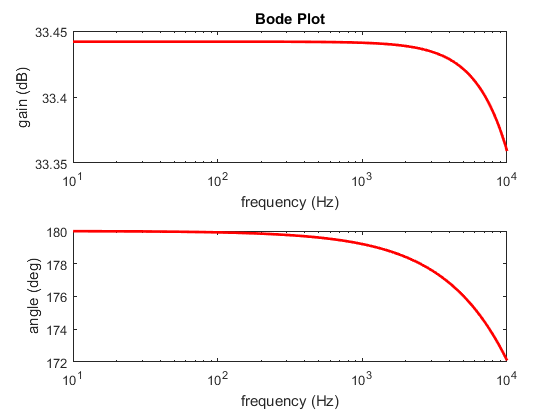
\includegraphics[width=\linewidth]{images/10.png}
			\caption{the Matlab Bode Plot for prelab \#10}
			\label{fig:1001}
		\end{framed}
	\end{figure}
	\section{\textbf{Prelab\#11}}
	\section{\textbf{Prelab\#12}}
	\section{\textbf{Prelab\#13}}
	\begin{eqnarray*}
		\frac{V_{in}}{\frac{1}{\mathbf{j}\omega C}} & + & \frac{V_{out}}{R_f}  =  0\\
		H(\mathbf{j}\omega) & = & \frac{V_{out}}{V_{in}}  =  -\mathbf{j}\omega CR_f
	\end{eqnarray*}
	\section{\textbf{Prelab\#14}}
	\section{\textbf{Prelab\#15}}
	\subsection{the Matlab Bode Plot}
	\begin{figure}[!htbp]
		\centering
		\begin{framed}
			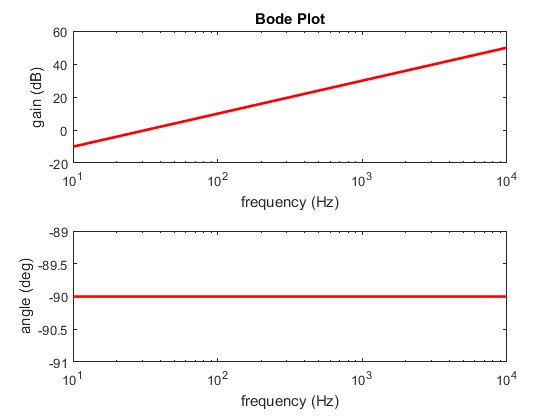
\includegraphics[width=\linewidth]{images/15.png}
			\caption{the Matlab Bode Plot for prelab \#15}
			\label{fig:1501}
		\end{framed}
	\end{figure}
\end{document}